\section{Test Results}
In this section, we test the proposed techinque on the use case explained in the previouse section.

\subsection{Verification of Results}
It is imporant to verify that the results obtained from the simulator actually matches real world observations.
Figure~\ref{} and~\ref{} show data from ???.

From Figure~\ref{fig:TestResults:distance0} we see that the simulation compared to the real-world results from Figure \ref{} is a close match. 
We see the same stop and go behavior as a results from traffic lights, and the arrival times are also a close match. 
If we compare the driving speed of the simulation show in Figure \ref{fig:TestResults:speed0} with the real-world data from Figure \ref{} we see that in most cases the vehicles are either driving at the maximum speed, or they are at a full stop. 
This behavior on the two graphs are almost identical and consistent with the stop and go behavior caused by traffic lights. 
Figure \ref{} shows the distance to a traffic light where each vehicles makes a stop. 
All the blue dots are vehicles that only have a single stop, red squares have two stops and yellow triangles have 3 stops.
The traffic light for this figure is the first junctions driving from Vesterbro. See Figure \ref{fig:Introduction:hobro}. The Figure \ref{} show the real-world data from the same traffic light. 
%TODO: when we have something to compare with

\begin{figure}[htb]
\includegraphics[width=0.5\textwidth]{images/tp0/speedUncontrolled0.png}
\caption{Speed graph}
\label{fig:TestResults:speed0}
\end{figure}

\begin{figure}[htb]
\includegraphics[width=0.5\textwidth]{images/tp0/distanceUncontrolled0.png}
\caption{Distance graph}
\label{fig:TestResults:distance0}
\end{figure}

%
\begin{figure}
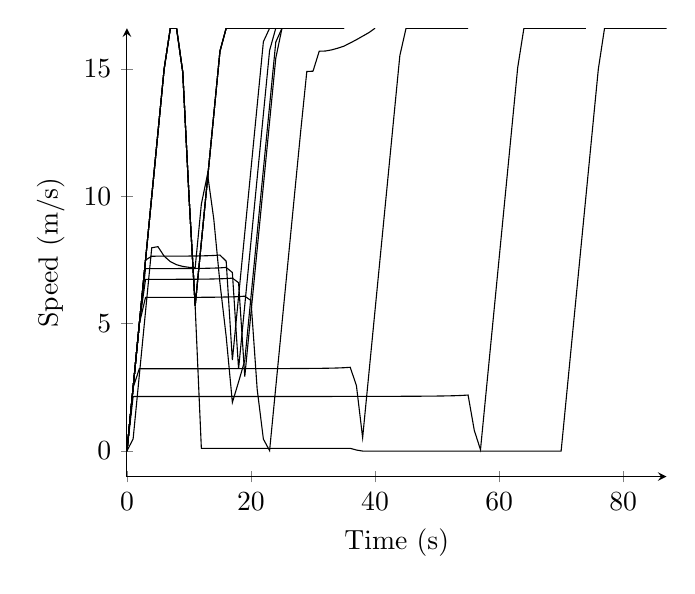
\begin{tikzpicture}
\begin{axis}[
legend style={anchor=west},
axis x line=bottom,
axis y line=left,
ymin=-1,
xlabel=Time (s),
ylabel=Speed (m/s),
]
\addplot[] coordinates {
(0, 0.0)
(1, 2.5)
(2, 5.0)
(3, 6.03141641743)
(4, 6.03166686901)
(5, 6.03195889103)
(6, 6.03230223965)
(7, 6.03270971778)
(8, 6.03319839585)
(9, 6.03379144568)
(10, 6.03452096802)
(11, 6.03543248316)
(12, 6.03659231065)
(13, 6.03810019083)
(14, 6.04011191689)
(15, 6.04411984346)
(16, 6.04833106741)
(17, 6.05430151178)
(18, 6.06397612583)
(19, 6.08136745541)
(20, 5.90769607444)
(21, 2.42026560792)
(22, 0.469751588191)
(23, 0.0183607863444)
(24, 2.51836078634)
(25, 5.01836078634)
(26, 7.51836078634)
(27, 10.0183607863)
(28, 12.5183607863)
(29, 14.9006120421)
(30, 14.9133190296)
(31, 15.6970460339)
(32, 15.7050303351)
(33, 15.749498614)
(34, 15.8174197091)
(35, 15.8973662005)
(36, 16.020950804)
(37, 16.1489838576)
(38, 16.2878875591)
(39, 16.4258529126)
(40, 16.6)
};
\addplot[] coordinates {
(0, 0.0)
(1, 0.480740698408)
(2, 2.98074069841)
(3, 5.48074069841)
(4, 7.98074069841)
(5, 8.02512604277)
(6, 7.6521410469)
(7, 7.43671687936)
(8, 7.31578448933)
(9, 7.249388471)
(10, 7.21388828355)
(11, 7.19592615636)
(12, 9.69592615636)
(13, 10.8759170188)
(14, 9.11147241477)
(15, 6.58947257263)
(16, 4.49910652234)
(17, 1.9093047889)
(18, 2.71553713327)
(19, 3.55698439678)
(20, 6.05698439678)
(21, 8.55698439678)
(22, 11.0569843968)
(23, 13.5569843968)
(24, 16.0569843968)
(25, 16.6)
(26, 16.6)
(27, 16.6)
(28, 16.6)
(29, 16.6)
(30, 16.6)
(31, 16.6)
(32, 16.6)
(33, 16.6)
(34, 16.6)
(35, 16.6)
};
\addplot[] coordinates {
(0, 0.0)
(1, 2.5)
(2, 5.0)
(3, 7.5)
(4, 10.0)
(5, 12.5)
(6, 15.0)
(7, 16.6)
(8, 16.6)
(9, 14.8767813611)
(10, 10.0411540628)
(11, 5.697212271)
(12, 8.197212271)
(13, 10.697212271)
(14, 13.197212271)
(15, 15.697212271)
(16, 16.6)
(17, 16.6)
(18, 16.6)
(19, 16.6)
(20, 16.6)
(21, 16.6)
(22, 16.6)
(23, 16.6)
(24, 16.6)
(25, 16.6)
(26, 16.6)
};
\addplot[] coordinates {
(0, 0.0)
(1, 2.5)
(2, 5.0)
(3, 7.5)
(4, 10.0)
(5, 12.5)
(6, 15.0)
(7, 16.6)
(8, 16.6)
(9, 14.8767813611)
(10, 10.0411540628)
(11, 5.697212271)
(12, 8.197212271)
(13, 10.697212271)
(14, 13.197212271)
(15, 15.697212271)
(16, 16.6)
(17, 16.6)
(18, 16.6)
(19, 16.6)
(20, 16.6)
(21, 16.6)
(22, 16.6)
(23, 16.6)
(24, 16.6)
(25, 16.6)
(26, 16.6)
};
\addplot[] coordinates {
(0, 0.0)
(1, 2.5)
(2, 5.0)
(3, 6.74095308203)
(4, 6.74126977766)
(5, 6.74164625624)
(6, 6.74209860481)
(7, 6.74264872435)
(8, 6.74332705456)
(9, 6.7441769198)
(10, 6.74526170501)
(11, 6.74667719459)
(12, 6.74857383207)
(13, 6.7511992742)
(14, 6.75668141598)
(15, 6.7624201969)
(16, 6.77181363873)
(17, 6.78892707945)
(18, 6.61062658727)
(19, 2.92750714793)
(20, 5.42750714793)
(21, 7.92750714793)
(22, 10.4275071479)
(23, 12.9275071479)
(24, 15.4275071479)
(25, 16.6)
(26, 16.6)
(27, 16.6)
(28, 16.6)
(29, 16.6)
(30, 16.6)
(31, 16.6)
(32, 16.6)
(33, 16.6)
(34, 16.6)
(35, 16.6)
};
\addplot[] coordinates {
(0, 0.0)
(1, 2.14203055668)
(2, 2.14205534875)
(3, 2.14208139585)
(4, 2.14210878425)
(5, 2.14213760776)
(6, 2.14216796856)
(7, 2.14219997811)
(8, 2.14223375816)
(9, 2.14226944191)
(10, 2.14230717538)
(11, 2.14234711888)
(12, 2.1423894487)
(13, 2.14243435915)
(14, 2.1424820647)
(15, 2.14253280269)
(16, 2.14258683618)
(17, 2.1426444575)
(18, 2.14270599217)
(19, 2.1427718036)
(20, 2.14284229845)
(21, 2.14291793307)
(22, 2.14299922089)
(23, 2.14308674131)
(24, 2.14318115012)
(25, 2.14328319198)
(26, 2.14339371532)
(27, 2.14351369026)
(28, 2.14364423024)
(29, 2.14378661833)
(30, 2.14394233935)
(31, 2.14411311934)
(32, 2.14430097445)
(33, 2.14450827181)
(34, 2.1447378059)
(35, 2.14499289527)
(36, 2.1452775059)
(37, 2.1455964101)
(38, 2.1463858743)
(39, 2.14687468003)
(40, 2.14733489185)
(41, 2.1478615681)
(42, 2.14846831318)
(43, 2.14917244958)
(44, 2.1499963276)
(45, 2.15096921683)
(46, 2.15213010086)
(47, 2.15353191577)
(48, 2.15524817652)
(49, 2.15738371252)
(50, 2.1600928189)
(51, 2.16361158715)
(52, 2.1683193786)
(53, 2.17486603603)
(54, 2.18446717344)
(55, 2.19971369605)
(56, 0.813780511493)
(57, 0.0549350715665)
(58, 2.55493507157)
(59, 5.05493507157)
(60, 7.55493507157)
(61, 10.0549350716)
(62, 12.5549350716)
(63, 15.0549350716)
(64, 16.6)
(65, 16.6)
(66, 16.6)
(67, 16.6)
(68, 16.6)
(69, 16.6)
(70, 16.6)
(71, 16.6)
(72, 16.6)
(73, 16.6)
(74, 16.6)
};
\addplot[] coordinates {
(0, 0.0)
(1, 2.5)
(2, 3.23233178617)
(3, 3.23239264744)
(4, 3.2324583658)
(5, 3.23252947295)
(6, 3.23260657547)
(7, 3.23269036792)
(8, 3.23278164862)
(9, 3.23288133883)
(10, 3.23299050629)
(11, 3.23311039409)
(12, 3.23324245651)
(13, 3.23338840369)
(14, 3.23355025777)
(15, 3.23373042397)
(16, 3.23393178137)
(17, 3.23415779997)
(18, 3.23441269294)
(19, 3.234701617)
(20, 3.23503093903)
(21, 3.23540859538)
(22, 3.23584458286)
(23, 3.23635163986)
(24, 3.23694620751)
(25, 3.23764981148)
(26, 3.23915888991)
(27, 3.24029909215)
(28, 3.24154219465)
(29, 3.24309038273)
(30, 3.2450541758)
(31, 3.24760025138)
(32, 3.25099053794)
(33, 3.25565837752)
(34, 3.26237010745)
(35, 3.27260956083)
(36, 3.28965750765)
(37, 2.56750741516)
(38, 0.526261895367)
(39, 3.02626189537)
(40, 5.52626189537)
(41, 8.02626189537)
(42, 10.5262618954)
(43, 13.0262618954)
(44, 15.5262618954)
(45, 16.6)
(46, 16.6)
(47, 16.6)
(48, 16.6)
(49, 16.6)
(50, 16.6)
(51, 16.6)
(52, 16.6)
(53, 16.6)
(54, 16.6)
(55, 16.6)
};
\addplot[] coordinates {
(0, 0.0)
(1, 2.5)
(2, 5.0)
(3, 7.16223631945)
(4, 7.16259645636)
(5, 7.16302958631)
(6, 7.16355690391)
(7, 7.16420791704)
(8, 7.16502470413)
(9, 7.16606896133)
(10, 7.16743415405)
(11, 7.16926750897)
(12, 7.17181221101)
(13, 7.17692719424)
(14, 7.1828538207)
(15, 7.19207571149)
(16, 7.20899763041)
(17, 7.00949388129)
(18, 3.22675481802)
(19, 5.72675481802)
(20, 8.22675481802)
(21, 10.726754818)
(22, 13.226754818)
(23, 15.726754818)
(24, 16.6)
(25, 16.6)
(26, 16.6)
(27, 16.6)
(28, 16.6)
(29, 16.6)
(30, 16.6)
(31, 16.6)
(32, 16.6)
(33, 16.6)
(34, 16.6)
};
\addplot[] coordinates {
(0, 0.0)
(1, 2.5)
(2, 5.0)
(3, 7.5)
(4, 7.65006899274)
(5, 7.65057209107)
(6, 7.65119399727)
(7, 7.65197540787)
(8, 7.65297612884)
(9, 7.65428699966)
(10, 7.65605154691)
(11, 7.65850769409)
(12, 7.66207417548)
(13, 7.66957454543)
(14, 7.67859691671)
(15, 7.69528048334)
(16, 7.45608012191)
(17, 3.57043002087)
(18, 6.07043002087)
(19, 8.57043002087)
(20, 11.0704300209)
(21, 13.5704300209)
(22, 16.0704300209)
(23, 16.6)
(24, 16.6)
(25, 16.6)
(26, 16.6)
(27, 16.6)
(28, 16.6)
(29, 16.6)
(30, 16.6)
(31, 16.6)
(32, 16.6)
(33, 16.6)
};
\addplot[] coordinates {
(0, 0.0)
(1, 2.5)
(2, 5.0)
(3, 7.5)
(4, 10.0)
(5, 12.5)
(6, 15.0)
(7, 16.6)
(8, 16.6)
(9, 14.8767813611)
(10, 10.0411540628)
(11, 5.697212271)
(12, 8.197212271)
(13, 10.697212271)
(14, 13.197212271)
(15, 15.697212271)
(16, 16.6)
(17, 16.6)
(18, 16.6)
(19, 16.6)
(20, 16.6)
(21, 16.6)
(22, 16.6)
(23, 16.6)
(24, 16.6)
(25, 16.6)
(26, 16.6)
};
\addplot[] coordinates {
(0, 0.0)
(1, 2.5)
(2, 5.0)
(3, 7.5)
(4, 10.0)
(5, 12.5)
(6, 15.0)
(7, 16.6)
(8, 16.6)
(9, 14.8767813611)
(10, 10.0411540628)
(11, 5.697212271)
(12, 0.105862141323)
(13, 0.105905445349)
(14, 0.105949933651)
(15, 0.105995655232)
(16, 0.106042661927)
(17, 0.106091008624)
(18, 0.106140753493)
(19, 0.106191958252)
(20, 0.10624468845)
(21, 0.106299013783)
(22, 0.106355008438)
(23, 0.106412751479)
(24, 0.106472327273)
(25, 0.10653382596)
(26, 0.10659734398)
(27, 0.106662984657)
(28, 0.106730858857)
(29, 0.106801085718)
(30, 0.106873793479)
(31, 0.106949120405)
(32, 0.107027215842)
(33, 0.1071082414)
(34, 0.107192372314)
(35, 0.10727979898)
(36, 0.107370728725)
(37, 0.0416172544952)
(38, 0.0)
(39, 0.0)
(40, 0.0)
(41, 0.0)
(42, 0.0)
(43, 0.0)
(44, 0.0)
(45, 0.0)
(46, 0.0)
(47, 0.0)
(48, 0.0)
(49, 0.0)
(50, 0.0)
(51, 0.0)
(52, 0.0)
(53, 0.0)
(54, 0.0)
(55, 0.0)
(56, 0.0)
(57, 0.0)
(58, 0.0)
(59, 0.0)
(60, 0.0)
(61, 0.0)
(62, 0.0)
(63, 0.0)
(64, 0.0)
(65, 0.0)
(66, 0.0)
(67, 0.0)
(68, 0.0)
(69, 0.0)
(70, 0.0)
(71, 2.5)
(72, 5.0)
(73, 7.5)
(74, 10.0)
(75, 12.5)
(76, 15.0)
(77, 16.6)
(78, 16.6)
(79, 16.6)
(80, 16.6)
(81, 16.6)
(82, 16.6)
(83, 16.6)
(84, 16.6)
(85, 16.6)
(86, 16.6)
(87, 16.6)
};
\addplot[] coordinates {
(0, 0.0)
(1, 2.5)
(2, 5.0)
(3, 7.5)
(4, 10.0)
(5, 12.5)
(6, 15.0)
(7, 16.6)
(8, 16.6)
(9, 14.8767813611)
(10, 10.0411540628)
(11, 5.697212271)
(12, 8.197212271)
(13, 10.697212271)
(14, 13.197212271)
(15, 15.697212271)
(16, 16.6)
(17, 16.6)
(18, 16.6)
(19, 16.6)
(20, 16.6)
(21, 16.6)
(22, 16.6)
(23, 16.6)
(24, 16.6)
(25, 16.6)
(26, 16.6)
};

\end{axis}
\end{tikzpicture}
\label{tik:100:53}
\caption{100 percent diving with GSC on route $53$}
\end{figure}

%
\begin{figure}
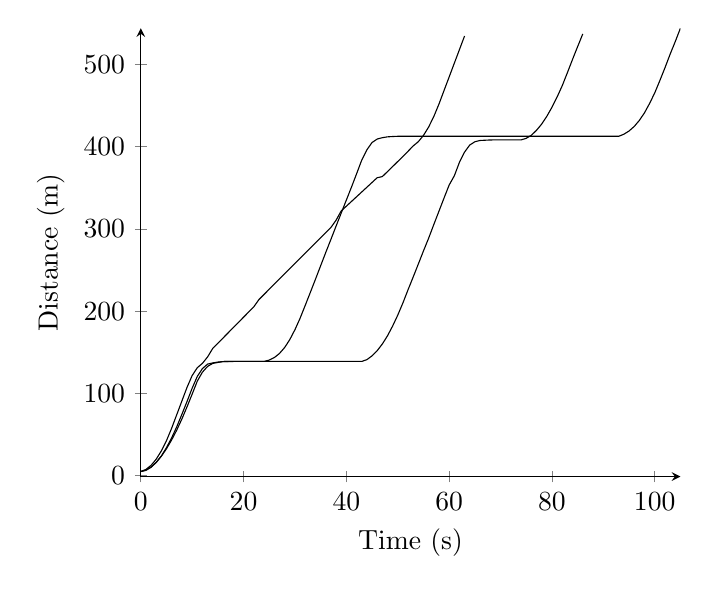
\begin{tikzpicture}
\begin{axis}[
legend style={
	anchor=west
},
axis x line=bottom,
axis y line=left,
ymin=-1,
point meta=explicit symbolic,
xlabel=Time (s),
ylabel=Distance (m)
]
\addplot[] coordinates {
(0, 5.1)
(1, 7.6)
(2, 12.6)
(3, 20.1)
(4, 30.1)
(5, 42.6)
(6, 57.6)
(7, 74.2)
(8, 90.8)
(9, 107.4)
(10, 121.758781889)
(11, 131.320742477)
(12, 136.609280481)
(13, 144.397818486)
(14, 154.68635649)
(15, 161.021784205)
(16, 167.357487819)
(17, 173.693488531)
(18, 180.029809771)
(19, 186.366477498)
(20, 192.703520555)
(21, 199.040971076)
(22, 205.378864977)
(23, 214.216758878)
(24, 220.474798436)
(25, 226.732975077)
(26, 232.991302485)
(27, 239.24979623)
(28, 245.508474103)
(29, 251.76735653)
(30, 258.026467073)
(31, 264.285833063)
(32, 270.54548638)
(33, 276.805464446)
(34, 283.065811483)
(35, 289.326580132)
(36, 295.58783356)
(37, 301.849648237)
(38, 310.611462913)
(39, 321.873277589)
(40, 327.639455454)
(41, 333.40702523)
(42, 339.176282693)
(43, 344.947614137)
(44, 350.721534016)
(45, 356.498743209)
(46, 362.280222462)
(47, 363.607388781)
(48, 369.687974655)
(49, 375.790220913)
(50, 381.925195852)
(51, 388.113297227)
(52, 394.397230867)
(53, 400.887229602)
(54, 406.011673174)
(55, 413.636116745)
(56, 423.760560316)
(57, 436.385003888)
(58, 451.509447459)
(59, 468.109447459)
(60, 484.709447459)
(61, 501.309447459)
(62, 517.909447459)
(63, 534.509447459)
};
\addplot[] coordinates {
(0, 5.1)
(1, 6.72319098396)
(2, 10.3468733498)
(3, 16.1332685505)
(4, 23.9286882805)
(5, 34.1720166711)
(6, 45.8890593831)
(7, 59.528275984)
(8, 74.6547246313)
(9, 90.2617056908)
(10, 106.406079189)
(11, 120.752868035)
(12, 130.281439818)
(13, 135.692922631)
(14, 137.147873208)
(15, 138.151456947)
(16, 138.752549833)
(17, 138.919508134)
(18, 138.930273837)
(19, 138.930273837)
(20, 138.930273837)
(21, 138.930273837)
(22, 138.930273837)
(23, 138.930273837)
(24, 138.930273837)
(25, 138.930273837)
(26, 138.930273837)
(27, 138.930273837)
(28, 138.930273837)
(29, 138.930273837)
(30, 138.930273837)
(31, 138.930273837)
(32, 138.930273837)
(33, 138.930273837)
(34, 138.930273837)
(35, 138.930273837)
(36, 138.930273837)
(37, 138.930273837)
(38, 138.930273837)
(39, 138.930273837)
(40, 138.930273837)
(41, 138.930273837)
(42, 138.930273837)
(43, 138.930273837)
(44, 141.114915808)
(45, 145.723578326)
(46, 151.998746932)
(47, 160.122800526)
(48, 170.022035583)
(49, 181.88207967)
(50, 195.182643297)
(51, 209.951444677)
(52, 226.009298917)
(53, 241.535058473)
(54, 257.259677345)
(55, 273.192092192)
(56, 288.571607169)
(57, 305.072725588)
(58, 321.279140443)
(59, 337.433303376)
(60, 353.346931963)
(61, 364.463502929)
(62, 380.895988341)
(63, 393.376922659)
(64, 401.949110189)
(65, 405.94426858)
(66, 407.522011955)
(67, 407.847468212)
(68, 408.163202868)
(69, 408.195381563)
(70, 408.195381563)
(71, 408.195381563)
(72, 408.195381563)
(73, 408.195381563)
(74, 408.195381563)
(75, 410.18501972)
(76, 413.845617016)
(77, 419.917654902)
(78, 427.393386755)
(79, 436.836262111)
(80, 447.819760421)
(81, 460.280904293)
(82, 474.035882427)
(83, 489.7969413)
(84, 505.936939978)
(85, 521.577093631)
(86, 537.018117137)
};
\addplot[] coordinates {
(0, 5.1)
(1, 6.52942920473)
(2, 10.397460774)
(3, 16.2332625509)
(4, 23.6898428533)
(5, 32.7746166262)
(6, 43.4439596056)
(7, 55.4796695473)
(8, 68.9530208007)
(9, 83.7525044986)
(10, 99.1987196739)
(11, 115.018047915)
(12, 125.904988034)
(13, 132.893465407)
(14, 136.539717246)
(15, 137.713754698)
(16, 138.775338083)
(17, 138.887378187)
(18, 138.919642787)
(19, 138.937871182)
(20, 138.937871182)
(21, 138.937871182)
(22, 138.937871182)
(23, 138.937871182)
(24, 138.937871182)
(25, 140.600580891)
(26, 143.690544118)
(27, 148.673520683)
(28, 155.907791651)
(29, 165.526496226)
(30, 177.544292589)
(31, 191.406263769)
(32, 207.110921725)
(33, 222.961991482)
(34, 239.000783121)
(35, 255.251148179)
(36, 271.513491617)
(37, 287.341622586)
(38, 303.408023612)
(39, 319.255356152)
(40, 335.112647816)
(41, 350.841227009)
(42, 367.19319554)
(43, 383.738226039)
(44, 396.198486332)
(45, 405.06887588)
(46, 409.280332872)
(47, 410.942766083)
(48, 411.946804448)
(49, 412.338587013)
(50, 412.617241737)
(51, 412.658060886)
(52, 412.658060886)
(53, 412.658060886)
(54, 412.658060886)
(55, 412.658060886)
(56, 412.658060886)
(57, 412.658060886)
(58, 412.658060886)
(59, 412.658060886)
(60, 412.658060886)
(61, 412.658060886)
(62, 412.658060886)
(63, 412.658060886)
(64, 412.658060886)
(65, 412.658060886)
(66, 412.658060886)
(67, 412.658060886)
(68, 412.658060886)
(69, 412.658060886)
(70, 412.658060886)
(71, 412.658060886)
(72, 412.658060886)
(73, 412.658060886)
(74, 412.658060886)
(75, 412.658060886)
(76, 412.658060886)
(77, 412.658060886)
(78, 412.658060886)
(79, 412.658060886)
(80, 412.658060886)
(81, 412.658060886)
(82, 412.658060886)
(83, 412.658060886)
(84, 412.658060886)
(85, 412.658060886)
(86, 412.658060886)
(87, 412.658060886)
(88, 412.658060886)
(89, 412.658060886)
(90, 412.658060886)
(91, 412.658060886)
(92, 412.658060886)
(93, 412.658060886)
(94, 415.153000888)
(95, 419.023672137)
(96, 424.501100973)
(97, 431.86335141)
(98, 441.039908442)
(99, 452.511470428)
(100, 465.308069565)
(101, 480.38143179)
(102, 496.032202461)
(103, 512.437839659)
(104, 527.797351639)
(105, 543.987083911)
};

\end{axis}
\end{tikzpicture}
\label{tik:50:12_O, 13_S, 15_N, 17_S, 17_S.-60, 19_V}
\caption{50 percent diving with GSC on route $12_O, 13_S, 15_N, 17_S, 17_S.-60, 19_V$}
\end{figure}

%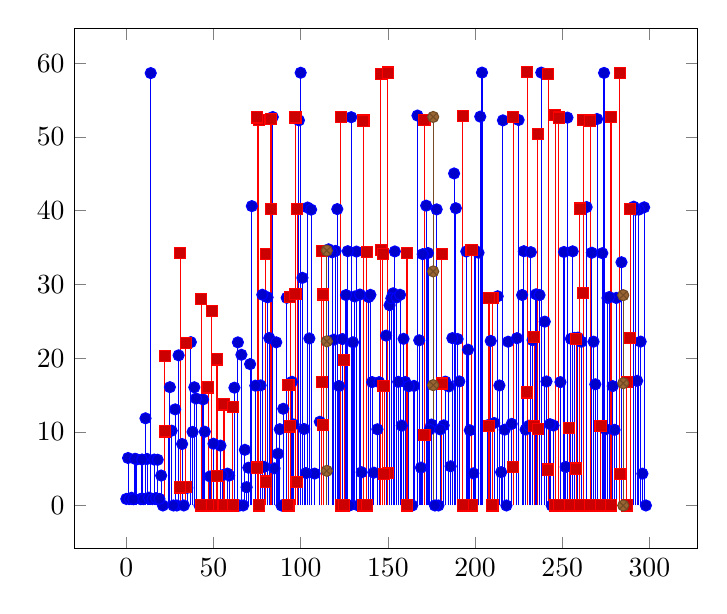
\begin{tikzpicture}\begin{axis} [width=9.5cm]
\addplot+[ycomb] coordinates{
(216, 52.252945617)
(217, 10.2835247016)
(214, 16.2856718575)
(215, 4.51864792679)
(213, 28.3873548357)
(211, 11.189338998)
(264, 40.4878802965)
(218, 0)
(219, 22.2220848566)
(133, 0)
(132, 34.4508958132)
(131, 28.3594198907)
(130, 22.1385166496)
(137, 0)
(135, 4.50616611369)
(165, 16.2267027888)
(139, 28.285187868)
(225, 52.3061097447)
(25, 16.0530002679)
(26, 10.1475132786)
(167, 52.905635371)
(20, 4.06070836139)
(21, 0)
(95, 16.7780005237)
(28, 13.0397800766)
(29, 0)
(178, 40.1749084596)
(0, 0.887926285604)
(221, 11.0667215168)
(281, 28.1590830651)
(8, 0.879701275233)
(96, 10.9849476286)
(284, 33.0003184931)
(68, 7.55165507934)
(87, 7.01750211778)
(119, 22.4988880985)
(263, 0)
(121, 40.2128463437)
(261, 22.2161474214)
(124, 22.5816882433)
(265, 0)
(127, 34.5048855528)
(128, 0)
(129, 52.6828088003)
(269, 16.4398851063)
(268, 22.2261723856)
(183, 16.8024845352)
(59, 4.06105996166)
(58, 4.32362219439)
(55, 4.10269772145)
(54, 8.12141482104)
(227, 28.5551151413)
(50, 8.38010669551)
(53, 0)
(259, 22.7745844792)
(298, 0)
(296, 4.31694972892)
(297, 40.4553565181)
(294, 40.1480987865)
(295, 22.2334499586)
(292, 40.1264458833)
(293, 16.9100041831)
(291, 40.5409654352)
(199, 4.35555745706)
(66, 20.4512404622)
(134, 28.6189430663)
(194, 0)
(197, 10.2047254435)
(196, 21.1414626766)
(191, 16.8319208832)
(190, 22.5846717422)
(271, 0)
(273, 34.2295001485)
(111, 11.3590799416)
(275, 10.3466370086)
(276, 28.1627318956)
(82, 22.718673814)
(279, 16.198959792)
(81, 28.2427318469)
(86, 22.1371668922)
(175, 10.9783281237)
(84, 52.7044109674)
(85, 5.04021199249)
(251, 34.3955366687)
(140, 28.580112231)
(108, 4.326167767)
(173, 34.2552838173)
(141, 16.7396435688)
(172, 40.6837062669)
(27, 0)
(3, 1.04420549155)
(255, 22.6172191574)
(24, 10.0531682208)
(245, 10.8464242737)
(244, 0)
(247, 0)
(241, 16.8271854495)
(240, 24.9439593649)
(243, 11.0294469892)
(102, 10.3777836793)
(103, 4.39269776309)
(100, 58.715030228)
(101, 30.8873579857)
(249, 16.738667879)
(104, 40.4248832298)
(105, 22.6658469812)
(39, 16.0389462527)
(38, 9.97543373366)
(33, 0)
(32, 8.33961614558)
(224, 22.6943008186)
(30, 20.3718391591)
(37, 22.1587029266)
(35, 2.38991943591)
(252, 5.22601443101)
(64, 22.13130224)
(65, 0)
(179, 0)
(67, 0)
(177, 0)
(69, 2.47903564849)
(174, 10.3127546711)
(256, 34.4823477755)
(257, 22.7308631355)
(170, 34.098783136)
(203, 52.7582624606)
(253, 52.6262542806)
(182, 10.8682501666)
(195, 34.4655481847)
(180, 10.3224731989)
(2, 0.889785751671)
(186, 5.31367419411)
(187, 22.7052298423)
(185, 16.1605886549)
(188, 45.0508173792)
(189, 40.3306851983)
(202, 34.2922024545)
(4, 0.858119596325)
(120, 34.5436475256)
(6, 6.26091222826)
(57, 0)
(99, 52.2575951587)
(168, 22.4135028295)
(169, 5.13775554004)
(229, 10.295455161)
(228, 34.5018262923)
(164, 0)
(92, 28.1764589812)
(160, 16.7564116485)
(162, 16.1825565598)
(11, 11.8283948176)
(10, 0.881112011558)
(13, 1.06146657052)
(12, 6.31020600882)
(15, 0.875296659051)
(14, 58.6672268685)
(17, 0.993840898557)
(16, 6.22794134696)
(19, 0.888781204593)
(18, 6.20293203127)
(118, 34.3543907429)
(88, 10.34819743)
(116, 34.7586327154)
(274, 58.6919651903)
(151, 27.1786828977)
(153, 28.7878919466)
(152, 28.1038034905)
(155, 28.2228618291)
(154, 34.4696486913)
(157, 28.5873349819)
(156, 16.775155837)
(159, 22.6084045705)
(158, 10.8361840758)
(62, 15.9833105543)
(277, 28.2764304681)
(90, 13.1217001857)
(238, 58.7327045428)
(235, 28.6501799394)
(237, 28.5527321263)
(231, 10.8267935469)
(232, 34.3695501862)
(233, 22.445048936)
(280, 10.2601636215)
(48, 3.93928596866)
(46, 0)
(44, 14.3903646534)
(45, 10.0088845232)
(42, 0)
(40, 14.5185355396)
(1, 6.44158771882)
(5, 6.33155562465)
(9, 6.23692159842)
(200, 34.5846228307)
(144, 10.3377609298)
(145, 16.728360112)
(142, 4.4518685762)
(204, 58.7375726484)
(207, 10.8693114242)
(209, 22.3262391201)
(149, 23.0494155894)
(77, 16.2953052439)
(74, 16.2546317465)
(106, 40.1412078513)
(72, 40.6167688582)
(71, 19.1793620961)
(70, 5.12135647663)
(79, 5.24282483604)
(78, 28.596095633)
(122, 16.2074955811)
(270, 52.4359425241)
(89, 0)
(267, 34.2918595684)
(126, 28.5503390242)};
\addplot+[ycomb] coordinates{
(210, 28.1097793763)
(210, 0)
(136, 52.2280479547)
(136, 0)
(138, 34.3467427786)
(138, 0)
(198, 34.6152811937)
(198, 0)
(22, 20.3266947089)
(22, 10.0447349346)
(289, 40.1976509476)
(289, 22.7168289734)
(283, 58.6320978831)
(283, 4.31438946042)
(123, 52.7292763657)
(123, 0)
(125, 19.7400405749)
(125, 0)
(56, 13.7112306443)
(56, 0)
(52, 19.8176908191)
(52, 4.04307309312)
(146, 58.5827933491)
(146, 34.6907037185)
(147, 34.1110400653)
(147, 16.2145455372)
(193, 52.8336680281)
(193, 0)
(80, 34.1002985828)
(80, 3.24308949069)
(254, 10.5251603275)
(254, 0)
(242, 58.5806667528)
(242, 4.87870006484)
(161, 34.2151874165)
(161, 0)
(34, 22.0585066331)
(34, 2.49293574307)
(246, 53.011035511)
(246, 0)
(94, 28.2491635302)
(94, 10.727029223)
(61, 13.312000988)
(61, 0)
(258, 22.6217152778)
(258, 5.01039621943)
(171, 52.3163917096)
(171, 9.55366723979)
(272, 10.8338464926)
(272, 0)
(181, 34.151374051)
(181, 16.5489447218)
(248, 52.6363940379)
(248, 0)
(97, 52.6547729656)
(97, 28.6648254432)
(98, 40.2593862116)
(98, 3.21946066682)
(222, 52.6819066117)
(222, 5.23552143383)
(93, 16.3158568778)
(93, 0)
(287, 16.7670833498)
(287, 0)
(31, 34.255056387)
(31, 2.44722481145)
(150, 58.7435786763)
(150, 4.41595408894)
(113, 28.6293422449)
(113, 10.9734549893)
(278, 52.6666260662)
(278, 0)
(83, 52.4478526303)
(83, 40.1971805753)
(234, 22.8473160709)
(234, 10.8390960135)
(236, 50.4031601251)
(236, 10.3285979681)
(230, 58.8696240113)
(230, 15.341659667)
(49, 26.3558240891)
(49, 0)
(47, 16.0158863142)
(47, 0)
(43, 27.9870688156)
(43, 0)
(208, 28.1330483343)
(208, 10.7370070602)
(148, 16.2311692676)
(148, 4.29963387855)
(76, 52.2595937482)
(76, 0)
(75, 52.6464795668)
(75, 5.15014459374)
(112, 34.4737051594)
(112, 16.80717737)
(262, 52.3174756198)
(262, 28.7833548519)
(260, 40.2876209009)
(260, 0)
(266, 52.2325690044)
(266, 0)};
\addplot+[ycomb] coordinates{
(285, 28.5350456998)
(285, 16.5886687888)
(285, 0)
(115, 34.5913828471)
(115, 22.27329098)
(115, 4.69795317646)
(176, 52.7187685594)
(176, 31.7604481719)
(176, 16.3285637619)
};
\end{axis}\end{tikzpicture}

\subsection{Fuel Consumption}
The purpose of \tech is to reduce the fuel consumption at least for the vehicles using the system. 
We use SUMO's build-in function to calculate the vehicles fuel consumption, which is explained in \cite{SUMOFuel}.


\begin{comment}
Figure~\ref{fig:TestResults:fuelRoute} plots the total fuel consumption for all vehicles driving on the selected route. 
The results clearly show that using \tech in this setup will reduce the fuel consumption significantly.
Acrose all routes, we see a reduction from an average of 130 $mL$ to an average of 96 $mL$, which is a reduction of 29 \%.
If we only look at route 1, we observe an average fuel consumption without \tech at 175 $mL$, and 117 $mL$ with \tech.
This is again a significant reduction in fuel consumption in 33 \%. %TODO fix number
\end{comment}

\begin{figure}[htb]
\includegraphics[width=0.5\textwidth]{images/tp0/fuelRouteControlled100.png}
\caption{Fuel graph}
\label{fig:TestResults:fuelRoute}
\end{figure}

\subsection{Distance}
Figure~\ref{fig:TestResults:distance100} shows the distance ?? vehicles drive on route 54 as a function of time when their driving behaviour is solely controled by SUMO. 
The vehicle is stationary whenever the curve flatens.
From the figure we clearly see that the vehicles on this route has to stop four times, at 250 meter, at 550 meters, at 750 meters and again at 1100 metets.

When we control the speed of the vehicles using \tech, we see a different result showed in Figure~\ref{fig:TestResults:distance100}.
The curves in this figure are much more smooth, and fewer vehicles has to stop completely at a cross section.
Some vehicles have to stop due to blocking vehicles or cross traffic, which we do not take into account.

We can therefore see that using \tech results in less full stops.


\begin{figure}[htb]
\includegraphics[width=0.5\textwidth]{images/tp0/distanceControlled100.png}
\caption{Distance graph}
\label{fig:TestResults:distance100}
\end{figure}

\subsection{Speed}
Figure~\ref{fig:TestResults:speed0} shows the speed at which SUMO controlled vehicles on route 54 drive as a function over time.
The graph clearly shows that the vehicles quicly accelerates up to the maximal speed, then quickly decelerates to a full stop and then quickly accelerates again.
By using \tech we see a very different outline (See Figure~\ref{fig:TestResults:speed100}).
Few vehicles decelerates to $0 m/s$, and many stay above $5 m/s$ ($18 km/h$ or $11$ miles per hour ($mph$)).
We do, however, still see a large fluctuation.
\begin{figure}[htb]
\includegraphics[width=0.5\textwidth]{images/tp0/speedControlled100.png}
\caption{Speed graph}
\label{fig:TestResults:speed100}
\end{figure}



\subsection{Time}
It is interesting to investigate wether driving after \tech results in longer travel time than without.
It takes on average 114 seconds to drive a route in our test without \tech, and when all vehicles drive with \tech it takes 111 seconds. 
We therefore do not see any significant differens in thees results.


